
\subsection*{1.}

\paragraph{a.}

\begin{center}
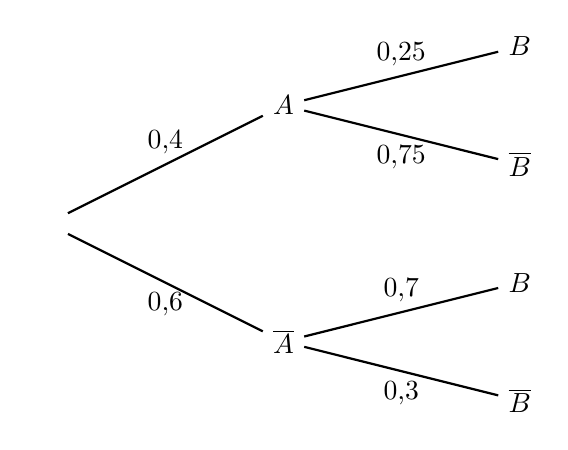
\begin{tikzpicture}[thick, scale=1.5]
\node (P_-1_0) at (-2,-1.5) {$\phantom{A}$};
\node (P_0_0) at (0,-0.5) {$A$};
\draw (P_-1_0) -- (P_0_0) node[midway, above] {$0{,}4$};
\node (P_1_0) at (2,-0) {$B$};
\draw (P_0_0) -- (P_1_0) node[midway, above] {$0{,}25$};
\node (P_1_1) at (2,-1) {$\overline{B}$};
\draw (P_0_0) -- (P_1_1) node[midway, below] {$0{,}75$};
\node (P_0_2) at (0,-2.5) {$\overline{A}$};
\draw (P_-1_0) -- (P_0_2) node[midway, below] {$0{,}6$};
\node (P_1_2) at (2,-2) {$B$};
\draw (P_0_2) -- (P_1_2) node[midway, above] {$0{,}7$};
\node (P_1_3) at (2,-3) {$\overline{B}$};
\draw (P_0_2) -- (P_1_3) node[midway, below] {$0{,}3$};
\end{tikzpicture}
\end{center}

\paragraph{b.} \(p(\overline{A} \cap \overline{B}) = p(\overline{A}) \times p_{\overline{A}}(\overline{B}) = 0{,}6 \times 0{,}3 = 0{,}18\).

La probabilité de choisir un chaton du second élevage et de couleur Chocolat est égale à \(0{,}18\).

\paragraph{c.} On a de même :
\[
p(A \cap \overline{B}) = p(A) \times p_A(\overline{B}) = 0{,}4 \times 0{,}75 = 0{,}3.
\]
D'après la loi des probabilités totales :
\[
p(\overline{B}) = p(\overline{A} \cap \overline{B}) + p(A \cap \overline{B}) = 0{,}18 + 0{,}3 = 0{,}48.
\]

\paragraph{d.} On calcule :
\begin{align*}
p_B(\overline{A}) &= \dfrac{p(B \cap \overline{A})}{p(B)} = \dfrac{p(\overline{A} \cap B)}{p(B)} \\
&= \dfrac{0{,}6 \times 0{,}7}{1 - 0{,}48} \\
&= \dfrac{0{,}42}{0{,}52} \approx 0{,}807,
\end{align*}
soit \(0{,}81\) au centième près.

La probabilité de choisir un chaton de couleur Blue à 100 € est égale à :
\[
p(X = 100) = 0{,}52,
\]
et la probabilité de choisir un chaton de couleur Chocolat est à 75 € est égale à :
\[
p(X = 75) = 0{,}48.
\]

